\chapter{Analisis dan Perancangan Sistem}

\section{Gambaran Umum Sistem}
Berikut Gambar \ref{fig:GambaranUmum} merupakan diagram blok dari sistem pakar yang dibangun:

\begin{figure}[h]	
	{\centering {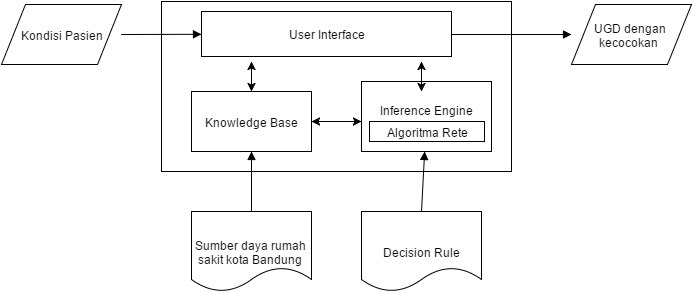
\includegraphics[scale=0.8]{gambaranUmum.png}}\par}
	\caption{Diagram Blok Gambaran Umum Sistem}
	\label{fig:GambaranUmum}
\end{figure}
Diagram blok pada Gambar \ref{fig:GambaranUmum} menggambarkan sistem dalam bekerja menerima input berupa kondisi pasien atau korban kejadian gawat darurat melalui interface sistem pakar. Knowledge base yang dibangun melalui metode pengumpulan data (observasi, wawancara pakar, studi literature) di intrepretasikan kedalam basis pengetahuan sistem pakar. Inference Engine dimana algoritma Rete diterapkan bertugas sebagai otak sistem pakar untuk melakukan pemilihan UGD berdasarkan rule dan knowledge base yang telah dibangun. \par
Berikut tahap dari pembangunan sistem pakar pemilihan UGD:
\begin{enumerate}
	\item Pembangunan knowledge base berupa informasi sumber daya rumah sakit di kota Bandung
	\item Menentukan kaidah pemilihan Unit Gawat Darurat untuk membangun decision rule yang digunakan dalam Inference Engine.
	\item Membangun inference engine dengan algoritma Rete
	\item Membangun user interface untuk menerima input berupa kondisi pasien dan menampilkan output berupa UGD dengan kecocokan yang dihasilkan oleh Inference Engine.
\end{enumerate} 
\par
Berikut simulasi menggambarkan bagaimana sistem yang dibangun bekerja akan diperlihatkan : 

\begin{figure}[h]	
	{\centering {\includegraphics[scale=0.9]{captureSimulasi.png}}\par}
	\caption{Simulasi sistem}
	\label{fig:simulasi}
\end{figure}
\par
Selanjutnya sistem akan memberikan lokasi dari Rumah Sakit yang merupakan keluaran dari sistem pakar, pada kasus ini adalah lokasi Rumah Bersalin Tunas Harapan yang diperlihatkan pada Gambar \ref{fig:hasil}. 
\begin{figure}[h]	
	{\centering \frame{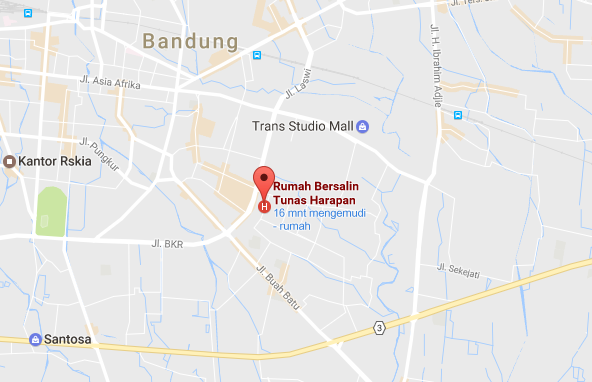
\includegraphics[scale=0.5]{hasilSistem.png}}\par}
	\caption{Lokasi RS UGD hasil keluaran sistem}
	\label{fig:hasil}
\end{figure}

\section{Data Kriteria}
Data kriteria pada tugas akhir ini merupakan data apa saja yang dijadikan pertimbangan dalam pemilihan Unit Gawat Darurat dalam suatu Rumah Sakit. Berdasarkan penelitian sebelumnya Weng dan Kuo \cite{weng2009} menggunakan kriteria ketersediaan dokter jaga, dokter bedah, dokter spesialis, ketersediaan ruang operasi dan kamar inap dan Jarak antara pasien dan lokasi UGD. Sedangkan Priyandari \cite{priyandari2011} melakukan perbaikan dengan mengganti jarak UGD menjadi waktu tempuh untuk menuju UGD. \par
Berdasarkan peraturan Kementrian Kesehatan RI \cite{kemenkes} dalam SPGDT (Sistem Penanggulangan Gawat Darurat Terpadu) telah diatur informasi data yang harus dikeluarkan oleh Rumah Sakit di Indonesia. Seperti data informasi fasilitas kesehatan terdekat, data informasi ketersediaan tempat tidur, ketersediaan Dokter, dll. Telah dilakukan penyeragaman kamus data antar Rumah Sakit sehingga dapat terhubung antar satu dan lainnya. Berikut Gambar \ref{fig:dataRS} adalah contoh data yang dikeluarkan oleh SPGDT:
\begin{figure}[h]	
	{\centering \frame{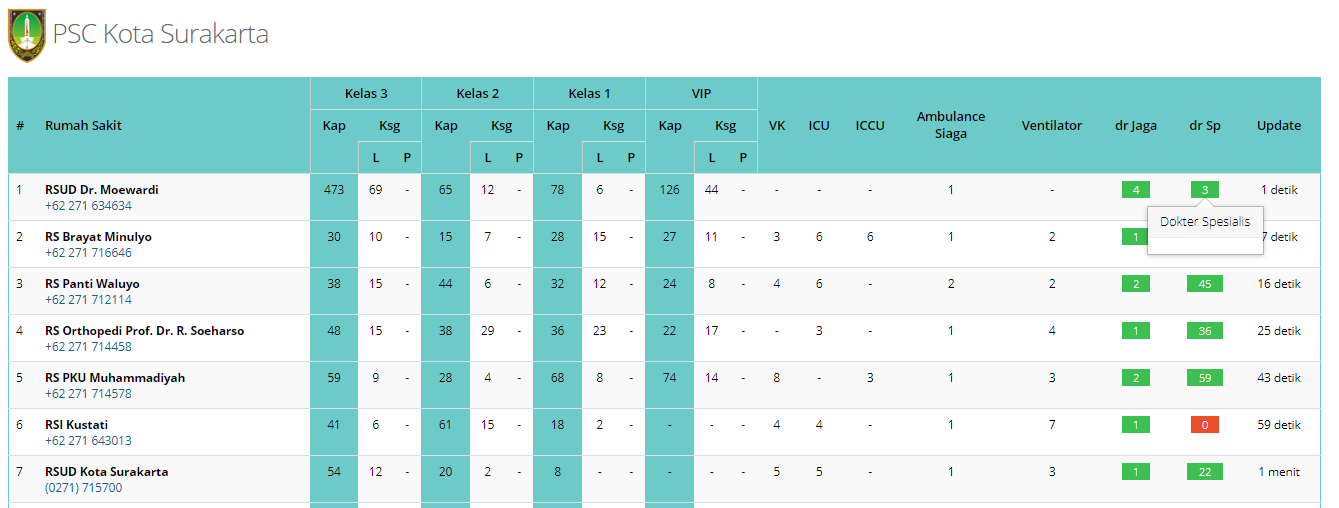
\includegraphics[scale=0.4]{dataRS.png}}\par}
	\caption{Data ketersediaan Rumah Sakit dari SPGDT}
	\label{fig:dataRS}
\end{figure}
\par
Keterangan untuk Gambar \ref{fig:dataRS}:
\begin{enumerate}
	\item Kap 	: Kapasitas 
	\item Ksg	: Kosong L/P
	\item VK		: Verlos Karmer (Ruang Bersalin)
	\item ICU	:  Intensif Care Unit
	\item ICCU	:  Intensif Cardiology Care Unit (Jantung)
	\item dr Jaga	: Doktek Jaga
	\item dr SP	: Dokter Spesialis
\end{enumerate}
\par
Dari data ketersedian fasilitas Rumah Sakit diatas system pakar yang dibangun diaharapkan dapat memilihkan UGD yang tepat sesuai kondisi pasien. Untuk data ketersedian Dokter jaga dan Dokter spesialis tersedia dalam SPGDT seperti terlihat dalam Gambar \ref{fig:dataDok} berikut :

\begin{figure}[h]	
	{\centering \frame{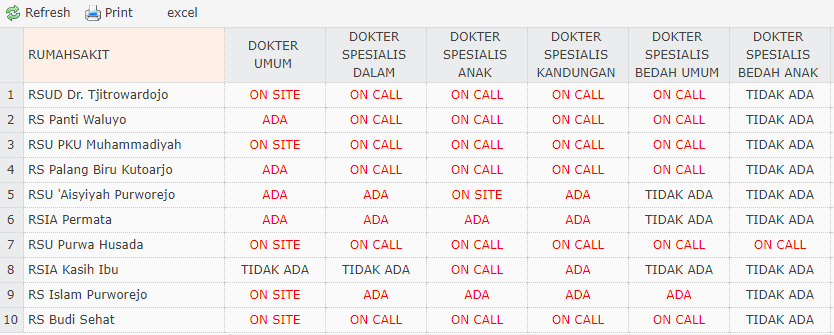
\includegraphics[scale=0.6]{dataDokter.png}}\par}
	\caption{Data ketersediaan Dokter Rumah Sakit dari SPGDT}
	\label{fig:dataDok}
\end{figure}

\par Dalam tugas akhir kriteria yang akan digunakan adalah ketersediaan ruang rawat inap ICU, ICCU, ruang operasi atau kamar bersalin. ketersediaan Dokter Spesialis, Kriteria kejadian berupa lokasi kejadiaan atau pasien dimana akan digunakan untuk menghitung waktu tempuh ke UGD. Untuk waktu tempuh didapat menggunakan Google Maps API V2.

\section{Uji Akurasi}
Hasil yang didapat berupa UGD yang terpilih oleh inference engine sesuai knowledge dan decision rule berdasarkan input kondisi pasien akan dibandingkan dengan pilihan dari pakar tenaga medis untuk mengetahui nilai akurasi sistem pakar pemilihan UGD yang dibangun dalam tugas akhir ini.

\section{Fungsional Sistem}
Fungsional sistem yang akan dibangun ini antara lain adalah :
\begin{enumerate}
	\item Sistem dapat menerima Input berupa kondisi calon pasien serta data kertersediaan Rumah Sakit
	\item Sistem dapat menampilkan lokasi UGD Rumah Sakit hasil keluaran sistem pakar
	\item Sistem dapat menerima inputan perbaikan aturan produksi sistem pakar dari user ahli
\end{enumerate}

\section{Deskripsi Lingkup Operasional}
Dalam penelitian ini, lingkup operasional yang digunakan baik itu perangkat
keras maupun perangkat lunak dijelaskan sebagai berikut:
\begin{enumerate}
	\item Spesifikasi Perangkat Keras\\
	Perangkat keras yang digunakan pada penelitian ini memiliki spesifikasi sebagai berikut :
	\begin{enumerate}
		\item Notebook Acer Aspire E5-553G-11Q
		\item AMD Quad-Core Processor A12-9700P 3.40 Ghz
		\item 8GB DDR4 Memory
	\end{enumerate}
	\item Spesifikasi Perangkat Lunak\\
	Perangkat lunak yang digunakan pada penelitian ini memiliki spesifikasi sebagai berikut :
		\begin{enumerate}
		\item Sistem Operasi Windows 10 Pro 64
		\item Sublime Text Editor
		\item Google Maps API V2
	\end{enumerate}
\end{enumerate}
